\section{Experiments} \label{sec:experiments}

\subsection{Training Environment and Hardware Specifications}

The model training was conducted within a Python Notebook environment
in Anaconda, utilizing PyTorch libraries with GPU acceleration.
The machine used features an AMD Ryzen 7 5800X CPU with 8 cores and
16 threads, operating at 4 GHz and
it is equipped with 16 GB of RAM running at 3600 MHz
and a PNY NVidia RTX 3070 graphics card with 8GB
of VRAM and 5888 CUDA cores.

\subsection{Training Process}

The model training process utilized a total of seconds,
as indicated in the following table:
\begin{table}[H]
    \centering
    \begin{tabular}{@{}lll@{}}
    \toprule
    Time (sec)               & \textbf{Age task} & \textbf{Gender task} \\ \midrule
    \textit{Single-task CNN} &  840.61           & 747.39               \\
    \textit{Multi-task CNN}  &  640.34           & *                    \\ \bottomrule
    \end{tabular}
\end{table}

Additionally, the epoch count for each training network is presented below:
\begin{table}[H]
    \centering
    \begin{tabular}{@{}lll@{}}
    \toprule
    Num. of epochs           & \textbf{Age task} & \textbf{Gender task} \\ \midrule
    \textit{Single-task CNN} & 8                 & 10                   \\
    \textit{Multi-task CNN}  & 9                 & *                    \\ \bottomrule
    \end{tabular}
\end{table}

In each training iteration, an early stopping mechanism was implemented with
a patience value set to 3 for both architectures.
The patience hyper-parameter was determined by monitoring the validation loss
of the model and stopping the training process when the loss
did not improve for a number of epochs equal to the patience value.

The training process was halted when the loss values
on the training set reached: 
\begin{table}[H]
    \centering
    \begin{tabular}{@{}lll@{}}
    \toprule
    Last loss value (training) & \textbf{Age task} & \textbf{Gender task} \\ \midrule
    \textit{Single-task CNN} &  0.5999           & 0.0027               \\
    \textit{Multi-task CNN}  &  1.2228           & *                    \\ \bottomrule
    \end{tabular}
\end{table}
and on the validation set:
\begin{table}[H]
    \centering
    \begin{tabular}{@{}lll@{}}
    \toprule
    Last loss value (validation) & \textbf{Age task} & \textbf{Gender task} \\ \midrule
    \textit{Single-task CNN} &  1.3413           & 0.0041               \\
    \textit{Multi-task CNN}  &  1.4058           & *                    \\ \bottomrule
    \end{tabular}
\end{table}
During the backpropagation, the loss value for the age task, 
was normalized by multiplying it by a factor
$\lambda_{\text{age}} = 0.01$.
By scaling down the loss for the age task, it effectively equalized
the magnitudes of both losses, ensuring a more balanced and comparable
training signal during the optimization process. 

In Fig.~\ref{1loss}, Fig.~\ref{2loss} and Fig.~\ref{3loss},
we can observe the trends through the iterations
of the loss
in the single task for age, the single task for gender
and the multi-task scenario, respectively.
In Fig.~\ref{4acc} and Fig.~\ref{5acc}, we can observe the
trends through the epochs of the accuracy
in the single task
and the multi-task scenario, respectively.

\begin{figure}[htbp]
    \centerline{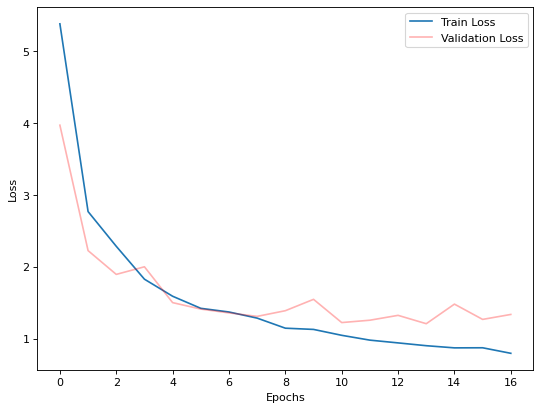
\includegraphics[width=.45\textwidth]{images/training/loss-single-age.png}}
    \caption{Loss trend in the single task for age}
    \label{1loss}
\end{figure}
\begin{figure}[htbp]
    \centerline{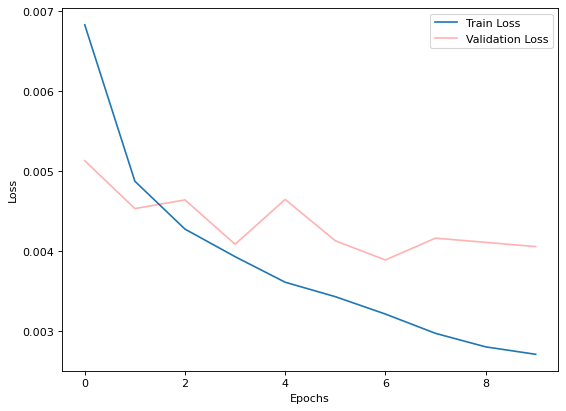
\includegraphics[width=.45\textwidth]{images/training/loss-single-gender.png}}
    \caption{Loss trend in the single task for gender}
    \label{2loss}
\end{figure}
\begin{figure}[htbp]
    \centerline{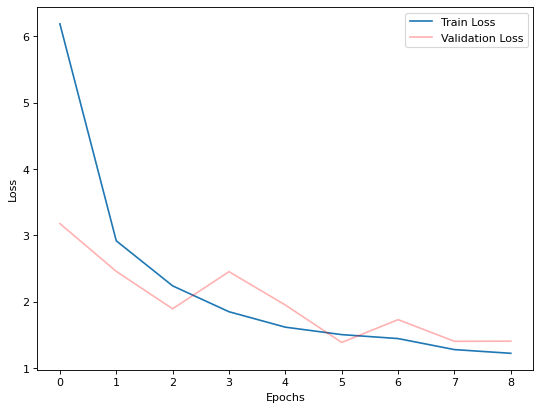
\includegraphics[width=.45\textwidth]{images/training/loss-multi.png}}
    \caption{Loss trend in the multi task}
    \label{3loss}
\end{figure}

\begin{figure}[htbp]
    \centerline{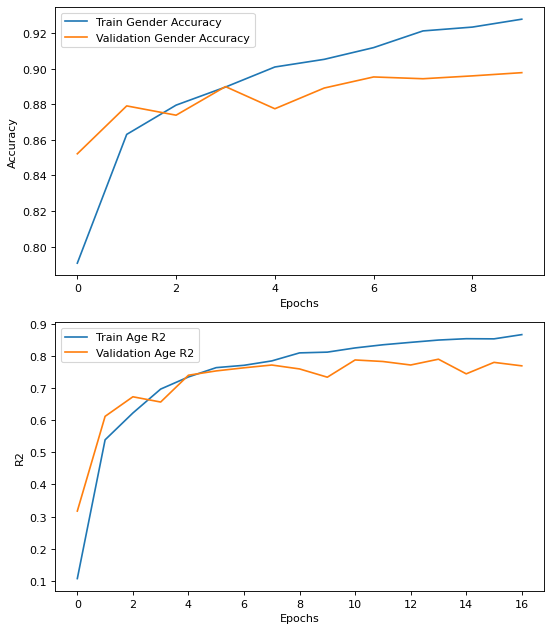
\includegraphics[width=.45\textwidth]{images/training/acc-single.png}}
    \caption{Accuracy trend in the single task CNNs}
    \label{4acc}
\end{figure}
\begin{figure}[htbp]
    \centerline{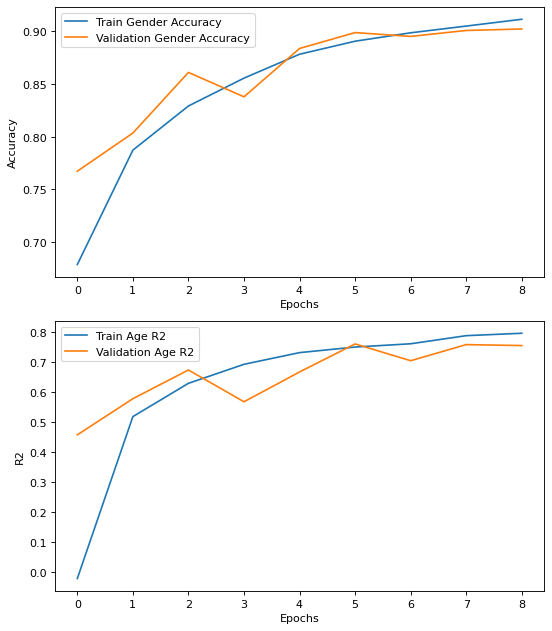
\includegraphics[width=.45\textwidth]{images/training/acc-multi.png}}
    \caption{Accuracy trend in the multi task CNN}
    \label{5acc}
\end{figure}

The training process ended with the following metrics on the training set:
\begin{table}[H]
    \centering
    \begin{tabular}{@{}lll@{}}
    \toprule
    Training Metrics & \textbf{Age task ($\mathbf{R^2}$)} & \textbf{Gender task (Accuracy)} \\ \midrule
    \textit{Single-task CNN} &                   &                      \\
    \textit{Multi-task CNN}  &                   &                      \\ \bottomrule
    \end{tabular}
\end{table}
and the following on the validation set:
\begin{table}[H]
    \centering
    \begin{tabular}{@{}lll@{}}
    \toprule
    Validation Metrics & \textbf{Age task ($\mathbf{R^2}$)} & \textbf{Gender task (Accuracy)} \\ \midrule
    \textit{Single-task CNN} &                   &                      \\
    \textit{Multi-task CNN}  &                   &                      \\ \bottomrule
    \end{tabular}
\end{table}

\subsection{Training Result}

After completing the model training, we can now transition to the testing
phase. During this phase, we load the testing images, which were initially
set aside without undergoing any preprocessing, and evaluate
the capabilities of the CNNs in explaining that data.
Below, you can find the table of accuracy and $R^2$ results for both
architectures:
\begin{table}[H]
    \centering
    \begin{tabular}{@{}lll@{}}
    \toprule
    Test Metrics & \textbf{Age task ($\mathbf{R^2}$)} & \textbf{Gender task (Accuracy)} \\ \midrule
    \textit{Single-task CNN} &                   &                      \\
    \textit{Multi-task CNN}  &                   &                      \\ \bottomrule
    \end{tabular}
\end{table}
along with Fig.~\ref{6mat} and Fig.~\ref{7mat} illustrating the
confusion matrices for single-task
and multi-task classification, respectively.
\begin{figure}[htbp]
    \centerline{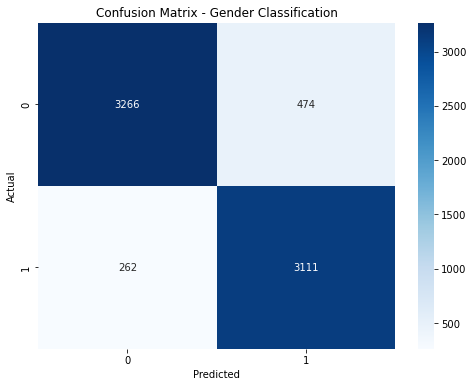
\includegraphics[width=.4\textwidth]{images/testing/mat_single.png}}
    \caption{Confusion Matrix for the single task}
    \label{6mat}
\end{figure}
\begin{figure}[htbp]
    \centerline{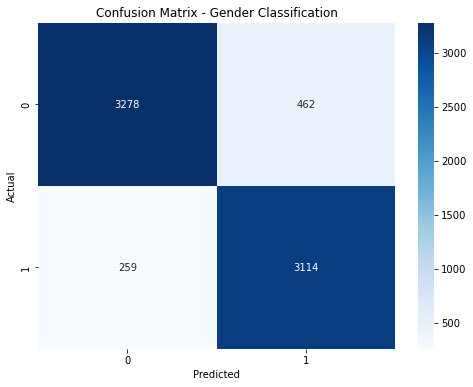
\includegraphics[width=.4\textwidth]{images/testing/mat_multi.png}}
    \caption{Confusion Matrix for the multi task}
    \label{7mat}
\end{figure}
To provide a visual example of the performance of the regressor,
we present, in Fig.~\ref{8reg} and Fig.~\ref{9reg},
a graph depicting the predicted age versus the ground truth
for both the single-task and multi-task scenarios for the first
50 observations of the set.
\begin{figure}[htbp]
    \centerline{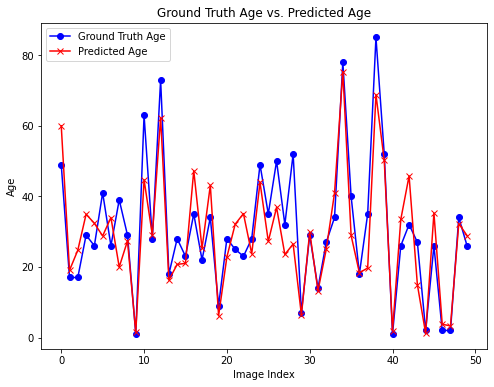
\includegraphics[width=.45\textwidth]{images/testing/reg_single.png}}
    \caption{Regressor performance example for the single task}
    \label{8reg}
\end{figure}
\begin{figure}[htbp]
    \centerline{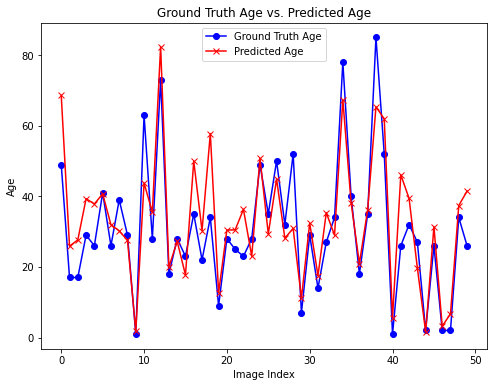
\includegraphics[width=.45\textwidth]{images/testing/reg_multi.png}}
    \caption{Regressor performance example for the multi task}
    \label{9reg}
\end{figure}

In the context of the provided example image in Fig.~\ref{1heat},
we can observe the corresponding mean attention heatmaps
for each convolutional layer in the neural network.
Specifically, Fig.~\ref{2heat} illustrates the single-task attention
heatmap for age, while Fig.~\ref{3heat} depicts the single-task
attention heatmap for gender and
Fig.~\ref{4heat} showcases the multi-task attention heatmap.
Notably, we can observe that the attention maps in the multi-task
scenario appear to be a weighted average,
with a notable bias towards the age-related features,
as compared to the two individual single-task scenarios.

\begin{figure}[htbp]
    \centerline{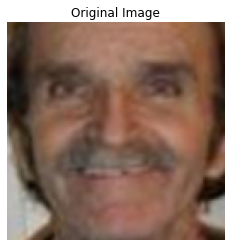
\includegraphics[width=.25\textwidth]{images/heatmaps/sample.png}}
    \caption{Sample image from the validation dataset}
    \label{1heat}
\end{figure}
\begin{figure}[htbp]
    \centerline{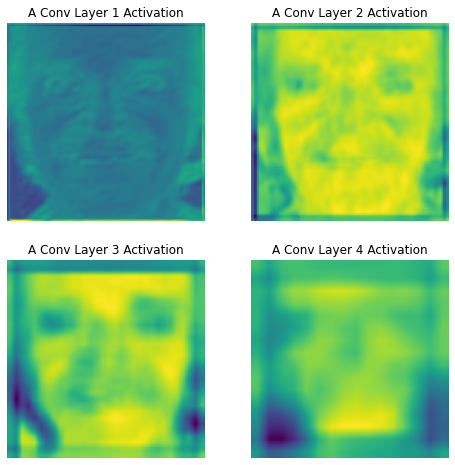
\includegraphics[width=.45\textwidth]{images/heatmaps/h_age.png}}
    \caption{Attention heatmap for the Age single-task CNN}
    \label{2heat}
\end{figure}
\begin{figure}[htbp]
    \centerline{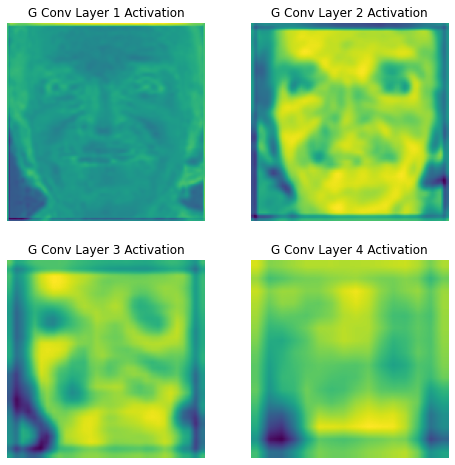
\includegraphics[width=.45\textwidth]{images/heatmaps/h_gender.png}}
    \caption{Attention heatmap for the Gender single-task CNN}
    \label{3heat}
\end{figure}
\begin{figure}[htbp]
    \centerline{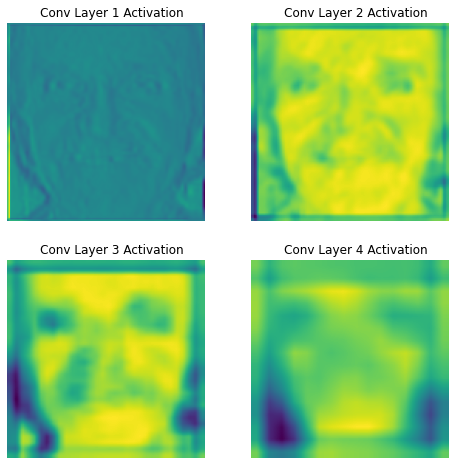
\includegraphics[width=.45\textwidth]{images/heatmaps/h_multi.png}}
    \caption{Attention heatmap for the multi-task CNN}
    \label{4heat}
\end{figure}